\documentclass[tikz]{standalone}

\usepackage{xcolor}
\colorlet{FilledSurface}{blue!20}
\colorlet{FilledSurfaceGroupOne}{blue!20}
\colorlet{FilledSurfaceGroupTwo}{red!20}
\colorlet{FilledSurfaceGroupThree}{green!20}
\colorlet{FilledSurfaceGroupFour}{magenta!20}
\colorlet{FormulaBackground}{green!10}
\colorlet{FormulaFrame}{green}


\usetikzlibrary{intersections, angles}

\begin{document}
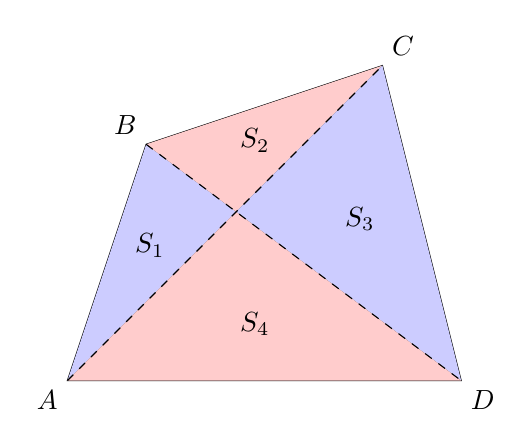
\begin{tikzpicture}

\coordinate (A) at (0, 0);
\coordinate (B) at (1, 3);
\coordinate (C) at (4, 4);
\coordinate (D) at (5, 0);
\draw[fill=blue!10!white]
    (A) node[below left]{$A$}
    -- (B) node[above left]{$B$}
    -- (C) node[above right]{$C$}
    -- (D) node[below right]{$D$}
    -- cycle;

\draw [name path=diagAC] (A) -- (C);
\draw [name path=diagBD] (B) -- (D);
\path [name intersections={of=diagAC and diagBD, by=P}];

\draw[draw=none, fill=FilledSurfaceGroupOne] (A) -- (B) -- (P) -- cycle;
\draw[draw=none, fill=FilledSurfaceGroupTwo] (B) -- (C) -- (P) -- cycle;
\draw[draw=none, fill=FilledSurfaceGroupOne] (C) -- (P) -- (D) -- cycle;
\draw[draw=none, fill=FilledSurfaceGroupTwo] (D) -- (A) -- (P) -- cycle;

\draw [dashed] (A) -- (C);
\draw [dashed] (B) -- (D);

\node at (barycentric cs:A=1,B=1,P=1) {$S_1$};
\node at (barycentric cs:B=1,C=1,P=1) {$S_2$};
\node at (barycentric cs:C=1,D=1,P=1) {$S_3$};
\node at (barycentric cs:A=1,D=1,P=1) {$S_4$};

\end{tikzpicture}
\end{document}
